\chapter{Theory and Background} \label{theoryandbg} 
This chapter overviews the background and main definitions and basic concepts, useful to the development of this investigation work.
\section{Learning environment}

	Learning environment refers to the diverse physical locations, contexts, and cultures in which students learn. Since students may learn in a wide variety of settings, such as outside-of-school locations and outdoor environments, the term is often used as a more accurate or preferred alternative to classroom, which has more limited and traditional connotations�a room with rows of desks and a chalkboard, for example.
The term also encompasses the culture of a school or class�its presiding ethos and characteristics, including how individuals interact with and treat one another�as well as the ways in which teachers may organize an educational setting to facilitate learning�e.g., by conducting classes in relevant natural ecosystems, grouping desks in specific ways, decorating the walls with learning materials, or utilizing audio, visual, and digital technologies. And because the qualities and characteristics of a learning environment are determined by a wide variety of factors, school policies, governance structures, and other features may also be considered elements of a �learning environment.�
Educators may also argue that learning environments have both a direct and indirect influence on student learning, including their engagement in what is being taught, their motivation to learn, and their sense of well-being, belonging, and personal safety. For example, learning environments filled with sunlight and stimulating educational materials would likely be considered more conducive to learning than drab spaces without windows or decoration, as would schools with fewer incidences of misbehavior, disorder, bullying, and illegal activity. How adults interact with students and how students interact with one another may also be considered aspects of a learning environment, and phrases such as �positive learning environment� or �negative learning environment� are commonly used in reference to the social and emotional dimensions of a school or class.

\section{Interactive learning environment}

	Interactive learning is a pedagogical approach that incorporates social networking and urban computing into course design and delivery. Interactive Learning has evolved out of the hyper-growth in the use of digital technology and virtual communication, particularly by students. The use of interactive technology in learning for these students is as natural as using a pencil and paper were to past generations. The Net Generation or Generation Y is the first generation to grow up in constant contact with digital media. Also known as digital natives, their techno-social, community bonds to their naturalized use of technology in every aspect of learning, to their ability to learn in new ways outside the classroom, this generation of students is pushing the boundaries of education. The use of digital media in education has led to an increase in the use of and reliance on interactive learning, which in turn has led to a revolution in the fundamental process of education.
Increasingly, students and teachers rely on each other to access sources of knowledge and share their information, expanding the general scope of the educational process to include not just instruction, but the expansion of knowledge. The role change from keeper of knowledge to facilitator of learning presents a challenge and an opportunity for educators to dramatically change the way their students learn. The boundaries between teacher and student have less meaning with interactive learning.
\section{Intelligent Tutoring System}

An intelligent tutoring system (ITS) is a computer system that aims to provide immediate and customized instruction or feedback to its learners during a task,[joseph p]without intervention from humans. ITSs have maintained the common goal of enabling learners to acquire information in a meaningful and effective manner by employing tools from a range of different technologies to direct the task at hand. There are numerous examples of ITSs being used in both education and professional settings since the mid-1920s. As a result, there is a strong relationship between ITSs, cognitive learning theories and instructional design. As with any mechanism for learning, ITSs have experienced its share of successes and limitations with continuous research investigating the best approach to addressing the dialogues and affective responses to learning.
Research in ITS organizes the "problem" in [1] knowledge about a domain, [2] knowledge about the learner, and [3] pedagogy (knowledge of teaching strategies). The major components of a typical ITS are an expert (or domain) model, student model and tutoring model. The expert model should be able to solve the problems the tutoring module submits to the students. The tutor module controls the interaction with the student, based on its teaching knowledge and comparisons between the student model and the domain knowledge. The student model reflects what the machine can infer about the student's cognitive state
\section{Intelligent learning environment}

An intelligent learning environment is a new kind of intelligent educational system, which combines the features of traditional Intelligent Tutoring Systems (ITS) and learning environments. An intelligent learning environment (ILE) includes special component to support student-driven learning, the environment module. The term environment is used to refer to that part of the system specifying or supporting the activities that the student does and the methods available to the student to do those activities [8]. Some recent ITS and ILE include also a special component called manual which provides an access to structured instructional material. The student can work with the manual via help requests or via special browsing tools exploring the instructional material on her own. An integrated ILE, which includes the environment and the manual components in addition to regular tutoring component, can support learning both procedural and declarative knowledge and provide both system-controlled and student-driven styles of learning.
\section{Fuzzy Logic}

	Zadeh introduced the term fuzzy logic in his work �fuzzy sets�, where he described the mathematics of the fuzzy set theory in 1965.
	Fuzzy logic gives the opportunity to model conditions that are defined with imprecision.
	The tolerance of the fuzzy in the process of human rezoning suggests that most of the logic behind the human rezoning is not the traditional bi-valued logic, or even the multi-valued, but the logic with fuzzy values, with fuzzy connections and fuzzy rules or inferences.

\subsection{Fuzzy sets}

	Fuzzy sets are an extension of the classic set theory and, as it name implies it, it is a set with boundaries not well defined, this means that the transition of belonging or not belonging to certain set is gradual, and this smooth transition is characterized by grades of membership that gives the fuzzy sets flexibility in modeling linguistic expressions commonly used, such as �the weather is cold� or �Gustavo is tall�.
 
Figure 2.1.Key-Value example.

\subsection{Fuzzy logic controller}

	Fuzzy control is a control method based on fuzzy logic. Just as fuzzy logic can be described simply as �computing with words rather than numbers� fuzzy control can be described simply as �control with sentences rather than equations�.
	The collection of rules is called a rule base. The rules are in the familiar if-then format, and formally the �if� side is called the antecedent and the �then� side is called the consequent.
	Fuzzy controllers are being used in various control schemes; the most used is the direct control, where the fuzzy controller is in the forward path in a feedback control system. The process output is compares with a reference, and if there is a deviation, the controller takes action according to the control strategy.
	In a feed forward control a measurable disturbance is being compensated, it requires a good model, but if a mathematical model is difficult or expensive to obtain, a fuzzy model may be useful. Fuzzy rules are also used to correct tuning parameters. If a nonlinear plant changes operating point it may be possible to change the parameters of the controller according to each operating point. His is called gain scheduling since it was originally used to change process gains. 
	A gain scheduling controller contains a linear controller whose parameters are changed as a function of the operating point in a preprogrammed way. It requires thorough knowledge of the plant, but it is often a good way to compensate for nonlinearities and parameter variations. Sensor measurements are used as scheduling variables that govern the change of the controller parameters, often by means of a table look-up.
\section{Learning object}


Learning object design raises issues of portability, and of the object's relation to a broader learning management system.
Learning objects are the basic elements of current Learning Management Systems (LMS) and are the focus of standardization initiatives whose goal is defining open technical standards and their characteristic metadata [6]. The most important initiatives are the Advanced Distributed Learning Initiative (ADL-SCORM) [7], the Instructional Management System Project (IMS) [8], the Alliance of Remote Instructional Authoring Distribution Networks of Europe (ARIADNE) [9], and the IEEE Learning Technology Standards Committee [10]. The main objective of these open standards is to enable the interoperability of learning objects between different LMSs and Learning Objects Repositories (LORS). Basic metadata schema specifications for learning objects include: Learning Object Metadata (LOM). Based on the Dublin Core metadata [11] this specification defines a set of meta- data elements that can be used to describe learning resources. LOM Includes educational, relation, technical, and classification elements [7]. Content Aggregation Model (CAM). CAM defines a package for the aggregation, distribution, management, and deployment of learning objects. Defines an organization element which contains information about one particular, passive organization of the material, the organization for now is limited to a tree structure [8]. Learner Information (LI). A collection of information about a learner or a producer of learning content, the elements are based upon accessibilities; activities; affiliations; competencies; goals; identifications; interests; qualifications, certifications and licenses; relationship; security keys; and transcripts [8]. Sequence and Navigation (SN). SN defines a method for representing the intended behavior of an authored learning experience such that any Learning Technology system (LTS) can sequence discrete learning activities in a consistent way. Provides a rule based sequencing of behaviors [7]. These standards have been the basis for various research projects in eLearning [11] and also extensions to support adaptability have been proposed [13], [14], [15]. Certain limitations of these specification initiatives have been noticed mainly regarding their weak support for the instructional design of the educational resources and pedagogy [16]. 

\section{Linda Spaces}

Linda [David Gelernter, 1985 Generative communication in Linda ACM Transactions on Programming Languages and Systems
Volume 7 , Issue 1 (January 1985), pp. 80-112] es un modelo que puede ser implementado para cualquier lenguaje que provea herramientas para crear y coordinar multiples procesos, algunas ejemplos de implementación son CppLINDA para C++, Simple C-Linda para C o PYLinda para Python. El concepto principal de LINDA es el de “Espacio de Tuplas” a través del cual los procesos se comunican. Este espacio de tuplas es una abstracción de un espacio de memoria compartida el cual se usa de manera asociativa.
El espacio de tuplas es donde se almacena la información accesible para todos los procesos. Las tuplas son colecciones de campos de algún tipo soportado por el lenguaje para el que se esta implementando. Estos campos pueden ser de dos tipos, valores de un tipo soportado o variables para recibir la información obtenida del espacio de tuplas, a las variables se les añade ? delante.
Habitualmente se definen tres operaciones sobre un espacio de
tuplas:
\begin{itemize}	
\item write(t) (out)
\begin{itemize}	
\item t es una tupla; el proceso deposita la tupla y sigue (no bloqueante)
\end{itemize}
\item take(p) (in)
\begin{itemize}
\item p es un patrón; el proceso se bloquea hasta que el espacio de tuplas le
asigna una que corresponda al patrón
\item la tupla es quitada del espacio de tuplas
\end{itemize}
\item read(p) (rd)
\begin{itemize}
\item versión del “take” en que la tupla que le es asignada no se elimina del
espacio de tuplas
\item puede haber varios read simultáneos
\end{itemize}
\end{itemize}
\begin{figure}[ht!]  
\centering  
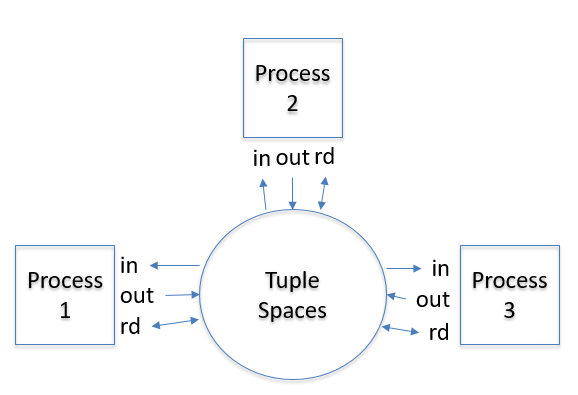
\includegraphics[scale=1]{linda}
\quad  
\caption{E-Learning}  
\label{keyvalue}  
\end{figure}

En el modelo básico las tuplas son bastante simples. Aqui se muestra una definicion general 
Let A be a set of typed elements, called atoms, for which a mapping.
 
\begin{equation}
EQ_{A} : A \times A \to \{ 0, 1 \} 
\end{equation}

%is assumed to be defined. The set of tuples TA is defined as follows: 
\begin{enumerate}	
\item for any a \( \in \) A, [a] belongs to \( \tau_{A} \)
%\item for any \[a\] \boldsymbol{\tau}_{A}, \[\[la\]\] belongs to \boldsymbol{\tau}_{A} 
%\item if [el] and [e2] belong to \boldsymbol{\tau}_{A}, then [e1 e2] also belongs to \boldsymbol{\tau}_{A}  
\end{enumerate}



\section{NoSQL}

In computing, NoSQL (sometimes called "not only SQL") is a broad class of systems management databases that differ from the classical model of relational database management system (RDBMS) in important aspects, the most prominent is that they are not using SQL as the primary query language. The stored data do not require fixed structures such as tables, typically do not support JOIN operations, not fully guarantee ACID (atomicity, consistency, isolation and durability), and usually scale well horizontally. The NoSQL systems are sometimes called "not only SQL" to underline the fact that they can also support query languages like SQL. The NoSQL databases Systems grew with major Internet companies like Google, Amazon, Twitter and Facebook. These had to face challenges with data processing than traditional RDBMS not solved. With the growth of the web in real time there was a need to provide processed information from large volumes of data that had more or less similar horizontal structures. These companies realized that the performance and real-time properties were more important than consistency, in which the traditional relational data bases devoted a lot of processing time. 
In that sense, often, NoSQL databases are highly optimized for operations retrieve and add, and usually do not offer much more than the functionality of store records (eg key-value storage) that we can see on figure \ref{keyvalue}. The loss of flexibility at run time compared to conventional systems SQL, is offset by significant gains in scalability and performance when it comes to certain data models.

 \begin{figure}[ht!]  
\centering  
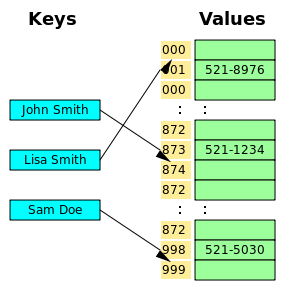
\includegraphics[scale=1]{nosqlejemplo}
\quad  
\caption{Key-Value Storage}  
\label{keyvalue}  
\end{figure}

\subsection{Key-Value example}

Typically the modern relational data bases have shown little efficiency in certain applications that use data intensively, including indexing of a large number of documents, presentation pages sites with high traffic, and sites audiovisual streaming. Typical implementations of RDBMS have tuned either for a small but frequent reads and writes or a large set of transactions that have few write accesses amount. On the other hand it can serve NoSQL lot of load of reads and writes.
\subsection{Advantages of NoSQL systems}

This way of storing information provides certain advantages over relational models. Between the most significant advantages can include:
They are executed in machines with limited resources: These systems, unlike based systems SQL, not just require computer, so they can be mounted on machines of a lower cost.
Horizontal Scalability: To improve the performance of these systems is achieved simply adding more nodes, with the only operation of the system indicate which nodes are available.
Can handle large amounts of data: This is because it uses a distributed structure, Hash many cases using tables.
Do not generate bottlenecks: The main problem with SQL systems is that they need to transcribe each sentence to be executed, and each complex sentence also requires a level even more complex implementation, which is an entry point in common, that before many requests can slow down the system.

\subsection{Main differences with SQL databases}

Some of the most remarkable differences we can find between NoSQL systems and SQL systems are:
Do not use SQL as a query language. Most NoSQL databases avoid using this kind of language or use it as a language support. To give some examples, Cassandra uses CQL language, MongoDB uses JSON or BigTable uses GQL.
Not use fixed structures as tables for storing data. Let you use other types of storage models as key-value systems, objects or graphs.
Tend not allow JOIN operations. By having a data volume so extremely large is often desirable to avoid the JOIN. This is because, when the operation is not the search for a key, the overhead can become very costly. The most straightforward solutions consist of denormalising data or perform the JOIN by software in the layer application.
Distributed architecture. The relational databases are typically centralized in a single machine or in a master-slave structure, however in cases NoSQL information it can be shared across multiple machines through mechanisms of distributed hash tables.

\subsection{Types of NoSQL databases}

Depending on how you store the information, we can find various types other than NoSQL databases. Consider the most commonly used types.
Key-Value Database: They are the base model popular NoSQL data, besides being the simplest in terms of functionality. In this type of system, each element is identified by a unique key, allowing the retrieval of information very quickly, which is usually stored information as a binary large object (BLOB). They are characterized by being very efficient for both readings and for scriptures. Examples of this type are Cassandra, HBase or BigTable.
 


Document databases: They are the base model popular NoSQL data, besides being the simplest in terms of functionality. In this type of system, each element is identified by a unique key, allowing the retrieval of information very quickly, which is usually stored information as a binary large object (BLOB). They are characterized by being very efficient for both readings and for scriptures we can see an example of this kind of data base on the figure 2.3. Examples of this type are Cassandra, HBase or BigTable. 
\begin{figure}[ht!]  
\centering  
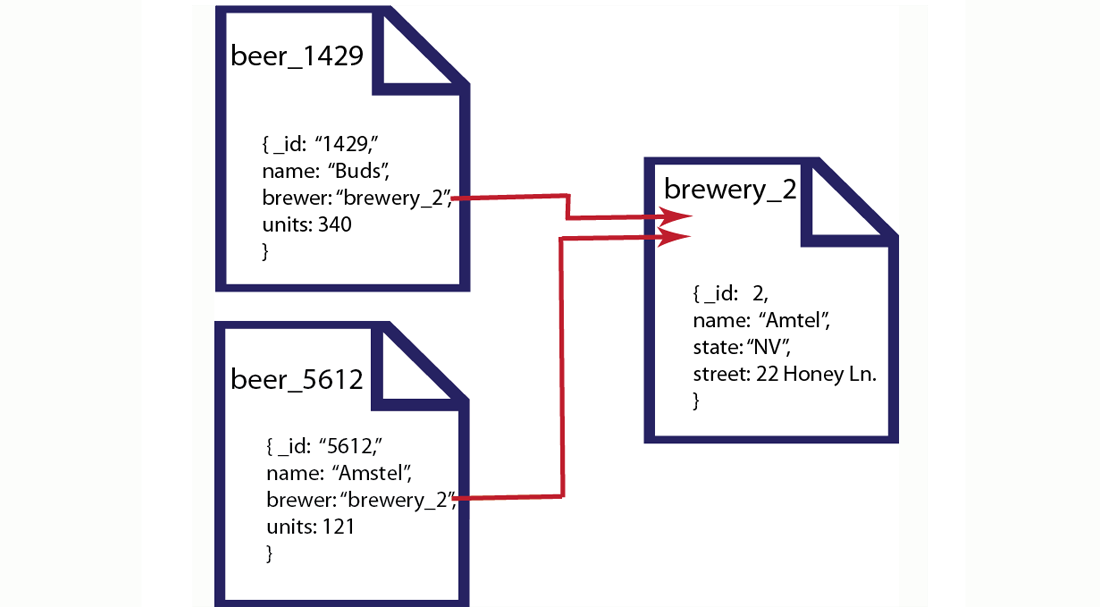
\includegraphics[scale=1]{basededatosdoc}
\quad  
\caption{Document Database Example}  
\label{bddd}  
\end{figure}

Graph databases: In this type of databases, information is represented as nodes of a graph and its relations with the edges thereof (Figure 2.4), so that you can make use of graph theory to cover it. To remove the most of this type of database, its structure must be fully normalized, of so that each table has a single column and each relationship both. This type of database provides a more efficient navigation between relationships vs a relational model. Examples of this type are Neo4j, InfoGrid or Virtuoso.

\begin{figure}[ht!]  
\centering  
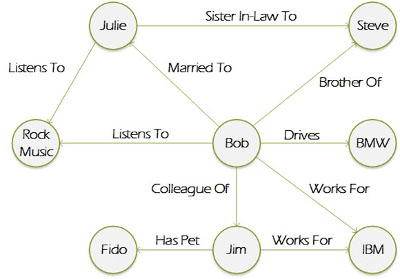
\includegraphics[scale=0.75]{Graph-database}
\quad  
\caption{Graph Database Example}  
\label{bdg}  
\end{figure}

\subsection{Examples of NoSQL databases}

Here are some examples of the most commonly used nosql databases.

Cassandra: This is a database created by Apache key-value type. It has its own language for CQL (Cassandra Query Language) queries. Cassandra is a Java application so it can run on any platform that has the Java Virtual Machine.
 
\begin{figure}[ht!]  
\centering  

\includegraphics[scale=0.1]{cassandra}
\quad  
\caption{Nosql Database Cassandra}  
\label{bdg}  
\end{figure}


MongoDB: This is a database created by 10gen document-oriented type, Free scheme is meaning that each input can have a different data schema that has nothing to do with the rest stored records. It's pretty quick to run its operations as it is written in C ++ language. For information storage, uses a proprietary system known document with the BSON name, which is an evolution of the popular JSON but with the peculiarity that can store binary data. Soon, MongoDB has become one of the bases of popular NoSQL data by developers.
 
\begin{figure}[ht!]  
\centering  

\includegraphics[scale=1]{mongo}
\quad  
\caption{Nosql Database MongoDB}  
\label{bdg}  
\end{figure}


CouchDB: It is a system created by Apache and written in Erlang language that works in most POSIX systems, including GNU / Linux and OSX, but not in Windows systems. The most important features include the use of Restfull HTTP API as an interface and JavaScript as the main language of interaction. For storage of data files used JSON.Allows creation of views, which are the mechanism that allows the combination of documents return values of several documents, ie, CouchDB allows performing operations JOIN Typical SQL.

\begin{figure}[ht!]  
\centering  

\includegraphics[scale=1]{couchdb}
\quad  
\caption{Nosql Database CouchDB}  
\label{bdg}  
\end{figure}

